%%%%%%%% mlsys 2021 EXAMPLE LATEX SUBMISSION FILE %%%%%%%%%%%%%%%%%

\documentclass{article}

% Recommended, but optional, packages for figures and better typesetting:
\usepackage{microtype}
\usepackage{graphicx}
% \usepackage{subfigure}
% \usepackage{booktabs} % for professional tables
% \usepackage{tabularx}
% \usepackage{tabu}
\usepackage{booktabs}% for better rules in the table
\graphicspath{ {./images/} }

% hyperref makes hyperlinks in the resulting PDF.
% If your build breaks (sometimes temporarily if a hyperlink spans a page)
% please comment out the following usepackage line and replace
% \usepackage{mlsys2021} with \usepackage[nohyperref]{mlsys2021} above.
\usepackage{hyperref}

% Attempt to make hyperref and algorithmic work together better:
\newcommand{\theHalgorithm}{\arabic{algorithm}}

% Use the following line for the initial blind version submitted for review:
% \usepackage{mlsys2021}

% If accepted, instead use the following line for the camera-ready submission:
\usepackage[accepted]{mlsys2021}

% The \mlsystitle you define below is probably too long as a header.
% Therefore, a short form for the running title is supplied here:
\mlsystitlerunning{CS/ECE/ME/EP 759 Final Project: Cautiously Aggressive GPU Space Sharing in Multi-Tenant Clusters}

\begin{document}

\twocolumn[
\mlsystitle{Cautiously Aggressive GPU Space Sharing in Multi-Tenant Clusters}

% It is OKAY to include author information, even for blind
% submissions: the style file will automatically remove it for you
% unless you've provided the [accepted] option to the mlsys2021
% package.

% List of affiliations: The first argument should be a (short)
% identifier you will use later to specify author affiliations
% Academic affiliations should list Department, University, City, Region, Country
% Industry affiliations should list Company, City, Region, Country

% You can specify symbols, otherwise they are numbered in order.
% Ideally, you should not use this facility. Affiliations will be numbered
% in order of appearance and this is the preferred way.
\mlsyssetsymbol{equal}{*}

\begin{mlsysauthorlist}
% \mlsysauthor{Aeiau Zzzz}{equal,to}
% \mlsysauthor{Bauiu C.~Yyyy}{equal,to,goo}
% \mlsysauthor{Cieua Vvvvv}{goo}
% \mlsysauthor{Iaesut Saoeu}{ed}
% \mlsysauthor{Fiuea Rrrr}{to}
% \mlsysauthor{Tateu H.~Yasehe}{ed,to,goo}
% \mlsysauthor{Aaoeu Iasoh}{goo}
% \mlsysauthor{Buiui Eueu}{ed}
% \mlsysauthor{Aeuia Zzzz}{ed}
% \mlsysauthor{Bieea C.~Yyyy}{to,goo}
% \mlsysauthor{Teoau Xxxx}{ed}
% \mlsysauthor{Eee Pppp}{ed}
\mlsysauthor{Rui Pan}{wisc}
\end{mlsysauthorlist}

% \mlsysaffiliation{to}{Department of Computation, University of Torontoland, Torontoland, Canada}
% \mlsysaffiliation{goo}{Googol ShallowMind, New London, Michigan, USA}
% \mlsysaffiliation{ed}{School of Computation, University of Edenborrow, Edenborrow, United Kingdom}
\mlsysaffiliation{wisc}{Department of Computer Science, University of Wisconsin-Madison, Madison, WI, United States}

\mlsyscorrespondingauthor{Rui Pan}{rpan33@wisc.edu}

% You may provide any keywords that you
% find helpful for describing your paper; these are used to populate
% the "keywords" metadata in the PDF but will not be shown in the document
\mlsyskeywords{Machine Learning, MLSys}

\vskip 0.3in

\begin{abstract}
Modern GPU architectures exhibit high versatility and specialization by including a myriad combination of cores (e.g., FP16, FP32, FP64) designed for different workloads. In current scheduling frameworks for large-scale multi-tenant GPU clusters, the scheduling/resource allocation model is leaving a large number of cores idle and not properly utilized. In this project, we first present a new insight into GPU utilization that takes into consideration the different types of cores utilized. Then, we improve the overall cluster utilization by breaking the current scheduling model and using aggressive space sharing of GPUs to pack multiple jobs on the same GPU concurrently with control over the resource partition fraction. Microbenchmarks show that for traces of common workloads, we are able to decrease the makespan by up to 30\% and the average job completion time (JCT) by up to 24\% compared to state-of-the-art (SOTA) GPU space sharing primitives.
% makespan when packing 7 jobs compared to 2: 2.47/1.76 = 1.4x, 0.71/2.47 = 30%
% jct table 2: 352.5/298.5 = 1.18  (15.3%)
% jct figure 1: 17/71 = 24%
\end{abstract}
]

\printAffiliationsAndNotice{} % otherwise use the standard text.

\section{Introduction}
\label{submission}

Recent years have seen an increase in high performance computing (HPC) and deep learning training (DLT) workloads. These workloads include both traditional HPC applications, like computational chemistry, financial risk modeling, and computer-aided engineering, as well as emerging applications, like machine learning, and deep learning, which widely cover tasks like image and voice recognition, language modeling and translation, recommendation systems, etc.

The foundation of the increasing popularity of these compute-intensive workloads is the emergence of specialized, domain-specific hardware accelerators, such as GPUs, TPUs \cite{tpu}, and FPGAs. Specifically, GPUs are designed to allow the faster computation of certain workloads by embracing specialized optimizations. These hardware accelerators are powerful yet expensive: A GPU virtual machine (VM) costs around 10x more than that of a regular VM. With different groups in the same organization running compute-intensive workloads, it is beneficial to consolidate GPU resources into a GPU cluster shared by multiple tenants. As a result of the high cost and the need for fair and efficient scheduling and resource allocation, it is crucial for cluster scheduling frameworks to ensure the proper utilization of hardware accelerators in the cluster.

One issue with fully utilizing GPU clusters is that the current model for estimating the utilization of GPUs is not precise enough: current GPU utilization monitoring tools do not provide a fine-grained estimation of the utilization of computing cores in a GPU. Modern GPU architectures exhibit high versatility by including a myriad combination of cores (FP16, FP32, FP64, etc.) designed for different workloads. However, almost all GPU utilization monitoring tools are wrapped around the NVIDIA System Management Interface (nvidia-smi) \cite{nvidia-smi}, which is developed on top of the NVIDIA Management Library (NVML) \cite{nvml}. The GPU utilization metric provided by NVML is a very coarse, upper-bound estimation of the utilization: it is defined as the “percent of the time over the past sample period during which one or more kernels was executing on the GPU”. As a result, at a certain point in time, as long as one kernel is being executed on the GPU, NVML considers the GPU to be fully utilized, while a lot of the cores may be sitting idle and are not being properly utilized. Some of the most recent works \cite{wavelet} report similar findings, in which occupancy rate replaces volatile GPU utility as the metric for monitoring utilization.


\begin{table*}[t]
\label{common-workloads}
\vskip 0.15in
\begin{center}
\begin{tabular*}{\textwidth}{@{\extracolsep{\fill}}|ccc|c|ccc|}
\toprule
Task & Model & Dataset & NVML Util & FP16 Util & FP32 Util & FP64 Util \\
\midrule
Image Classification & ResNet-18 & CIFAR10 & 76.8\% & 0\% & 40.26\% & 0\% \\
Image Classification & ResNet-18 Q & CIFAR10 & 47.5\% & 30.05\% & 32.36\% & 0.38\% \\
Image Classification & ResNet-50 & ImageNet & 96.4\% & 0\% & 52.02\% & 0.02\% \\
Language Modeling & LSTM & Wikitext-2 & 73.5\% & 0\% & 33.04\% & 0\% \\
Language Modeling & LSTM Q & Wikitext-2 & 62.9\% & 11.34\% & 11.44\% & 0\% \\
Recommendation & Recoder & ML-20M & 12.2\% & 0\% & 24.97\% & 0\% \\
cuBLAS DGEMM & N/A & Synthetic matrices & 84.72\% & 0\% & 0\% & 59.78\% \\  % measurement done
\bottomrule
\end{tabular*}
\end{center}
\caption{Common DL/HPC workloads used in the evaluation. The "Q" indicates quantization/mixed precision training \cite{mixed_precision}. In this project, we use NVIDIA Apex \cite{apex} and PyTorch AMP \cite{amp} for quantization. "NVML Util" indicates the GPU utilization as reported by NVML averaged over time. "FP Util" indicates the core utilization as measured by the profiler wrapper we developed.}
\vskip -0.1in
\end{table*}






To tackle this issue, we break the traditional resource allocation model in shared clusters and use aggressive space sharing of GPUs to pack/co-locate multiple jobs on the same GPU concurrently. Traditionally, GPUs are considered as bulky hardware that is not easily virtualizable and shared. In recent years, however, the improvements in both GPU architectures and software support are slowly breaking apart this notion. With the NVIDIA Multi-Process Service (MPS), the sharing of a single GPU context by multiple CUDA processes, "space sharing (SS)", is better supported, particularly in post-Volta architectures. 

Some of the most cutting-edge scheduling frameworks and policies already take into consideration the space sharing of multiple jobs on the same GPU. However, they have some shortcomings that result in the sub-optimal resource utilization of GPUs and efficiencies of jobs. In this project, we present techniques such as fine-grained fractional space sharing and aggressive multi-job space sharing to address these problems.

As an overview, this report:
\begin{itemize}
\item Provides a better understanding of GPU utilization that takes into consideration the utilization of different types of cores, rather than the current, coarse estimation provided by GPU monitoring tools (§3)
\item Presents a profiler that is built around NVIDIA Visual Profiler which reports the utilization of different types of cores of workloads (§3)
\item Presents a Python interface for interacting with NVIDIA Multi-Process Service (MPS) \cite{mps} that is uploaded to the Python Package Index for public use (§3)
\item Reports a fine-grained profiling of how different GPU cores get utilized in common DL/HPC workloads (§4.1)
\item Reports microbenchmarks that show how cautiously aggressive space sharing (using fine-grained fractional SS \& aggressive multi-job SS) improves the resource utilization of a GPU and the avg JCT \& makespan of a trace of jobs (§4.2 - 4.4)
\end{itemize}

The results in this report can be replicated by following the instructions in the Appendix.

\begin{figure*}
\label{ss_benefits}
    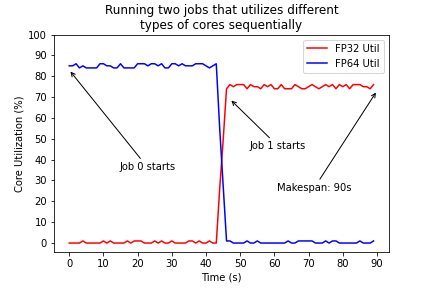
\includegraphics[width=.33\textwidth]{images/fig1_fifo.png}\hfill
    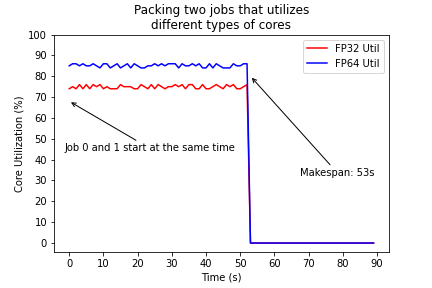
\includegraphics[width=.33\textwidth]{images/fig1_ss.png}\hfill
    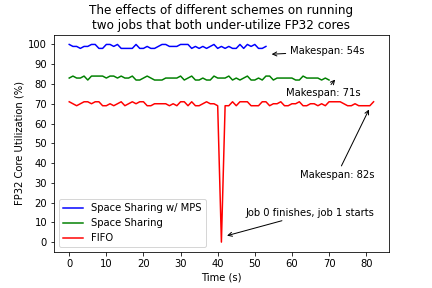
\includegraphics[width=.33\textwidth]{images/fig1a.png}\hfill
    % \\[\smallskipamount]
    \caption{Visual illustration of the benefits of space sharing. Left \& Middle: Running two jobs that utilize different types of cores using FIFO (left) and Space Sharing w/ MPS (middle). Right: Running two jobs that both under-utilize FP32 cores using different schemes.}
    \label{fig:foobar}
\end{figure*}



\section{Background}

In this section, we provide a brief overview of common DL/HPC workloads (§2.1), popular GPU profiling and monitoring tools (§2.2), and existing GPU space sharing primitives (§2.3).

\subsection{Common Deep Learning and High Performance Computing Workloads}

In this section, we give a brief overview of the common DL/HPC workloads and their characteristics.

Deep learning and deep neural networks (DNNs) are revolutionizing all subject areas. We excerpt a trace of common DNN workloads from Gavel \cite{gavel}, where ResNet-18 and ResNet-50 \cite{resnet} are used for image classification workloads, LSTM \cite{lstm} is used for language modeling workloads, and Recoder/Autoencoder \cite{recommendation} is used for Recommendation workloads. The standard precision for DNN workloads has long been single precision (FP32). In recent years, there has been a trend to use mixed precision training (quantization) \cite{mixed_precision} which replaces some CUDA kernels that run on FP32 cores with kernels that utilize FP16 (half precision) tensor cores. Mixed-precision training brings a significant speedup to the training time without any adversarial effects on accuracy, and it also reduces the memory consumption of a DNN training job.

In high performance computing and scientific computations with rather strong precision requirements, except from FP16 and FP32, the double-precision (FP64) format is also used, as low precision floating formats are not precise enough and lead to accumulation of errors. In this project, we use the cuBLAS \cite{cublas} DGEMM function to emulate a HPC workload, where we apply the function on synthetic 512*512 matrices.

A list of DL/HPC workloads this project uses for evaluations can be found in Table \ref{common-workloads}.


\subsection{GPU Profiling and Monitoring Tools}

\textbf{NVIDIA Management Library (NVML):} NVML \cite{nvml} is a C-based API for monitoring and managing various states of the NVIDIA GPU devices. It provides a direct access to the queries and commands exposed via nvidia-smi. One of the most used metric that is query-able by NVML is GPU utilization (Volatile-GPU-Util). NVML defines GPU utilization to be the "percent of time over the past sample period during which one or more kernels was executing on the GPU", making this a coarse-grained, upper-bound estimation of the utilization of different types of cores in the whole GPU. 

\textbf{NVIDIA System Management Interface (nvidia-smi):} nvidia-smi \cite{nvidia-smi} is a command line utility, based on top of NVML, intended to aid in the management and monitoring of NVIDIA GPU devices. This utility allows the querying of GPU device state.

\textbf{NVIDIA Visual Profiler (nvprof \& nvvp):} The NVIDIA Visual Profiler \cite{nvprof} is a cross-platform performance profiling tool that delivers developers vital feedback for optimizing CUDA C/C++ applications. nvprof operates in one of the four modes: summary mode, GPU-Trace and API-Trace modes, event/metric summary mode, event/metric trace mode.
% The NVIDIA Visual Profiler (nvprof) provides a utility to turn on/off concurrent kernel execution. If this option is turned on, all kernels running on one device will not be serialized. However, note that nvprof has three profiling use cases (Timeline, Metrics and Events, Analysis for Individual Kernel) and only the Timeline mode supports concurrent kernel execution. Although the metric/event collection mode serializes all kernel execution and significantly impacts the overall performance, the event/metric values for individual kernels are all correct, so it is possible to merge the event/metric values onto a previously collected timeline to get an accurate picture of the application behavior.


\textbf{NVIDIA NSight Compute + Nsight Systems:} The NVIDIA Volta platform is the last architecture on which the NVIDIA Visual Profiler tools are fully supported. Nsight Systems \cite{nsight_systems} is now used for GPU and CPU sampling and tracing to provide comprehensive system-wide, workload-level application performance, and Nsight Compute \cite{nsight_compute} is used for GPU kernel profiling by providing detailed performance metrics analysis and debugging on GPU CUDA kernels.


% \subsection{Common Policies and the Metrics to Evaluate their Effectiveness}
% fifo, sjf, srtf, allox, las, drf, themis, ...



\subsection{Existing GPU Space Sharing Primitives}

% give the definition of {avg jct, makespan, fairness} in this section


% Gandiva: trial-and-error, instead of making decisions before dispatching the scheduled jobs
% Gavel: only packs 2 jobs but not more; no control over fractional resource partition; relies on pre-profiling of all jobs???
% note: more jobs = more pre-profiling in gavel


\textbf{Gandiva:} The space sharing policy in Gandiva \cite{gandiva} uses profiling to approximate the resource usage (GPU utilization, GRAM usage \& job progress rate) before greedily packing jobs with the lowest GPU utilizations on a GPU with the lowest utilization. If the two jobs packed adversely impact each other (indicated by the total throughput of packed jobs being lower than that of time slicing), Gandiva retracts the packing decision and attempts to use the GPU with the next lowest utilization. Gandiva uses this simple heuristic because analytically modeling performance of packing is challenging given the heterogeneity of DLT jobs, and the inter-job interference may come from various sources like caches and memory bandwidth, etc. Gandiva does not provide an open-sourced implementation, but its scheduling policies are emulated in Gavel as optimization problems.

% \textbf{Tiresias:} The main contribution of Tiresias is two scheduling algorithms that minimize the average job completion time (JCT). The scheduler takes into consideration the placement sensitivity of distributed jobs when allocating resources. Neither time sharing nor space sharing are used.

% \textbf{Themis:} Themis proposes a new fairness objective, finish-time fairness, and an auction-based scheduler to improve both fairness and efficiency. Themis also considers the placement sensitivity. Themis does not incorporate time sharing or space sharing.

\textbf{Salus:} Salus \cite{salus} presents two GPU sharing primitives for fine-grained GPU sharing among multiple DL applications: fast job switching (for time-sharing and preemption) and GPU lane abstraction (for dynamic memory sharing). The GPU lane abstraction divides the GPU memory space into continuous memory spaces  (lanes), which allows for time-slicing within lanes and parallelism across lanes. Salus also supports automatic in-lane defragmentation and dynamic lane assignment (re-partitioning).

\textbf{Gavel:} Gavel \cite{gavel} takes into consideration the heterogeneous performance of DLT jobs on different hardware accelerators because of the difference in the model architectures. Gavel expresses scheduling policies as optimization problems and produces allocations as time fractions. On top of time sharing in the form of time fraction matrices, Gavel's policies can incorporate space sharing to consider job combinations of at most two jobs.

\begin{table*}[t]
\label{mps_weight_tuning}
\vskip 0.15in
\begin{center}
% \begin{small}
\begin{tabular*}{\textwidth}{@{\extracolsep{\fill}}|c|cc|cc|cc|}
% \begin{center}
\toprule
Sharing Scheme & Job 1 Run Time & Job 2 Run Time & Job 1 JCT & Job 2 JCT & Avg JCT & Makespan \\
\midrule
FIFO & 316 & 144 & 316 & 460 & 388 & 460\\
Space Sharing w/o MPS & 405 & 202 & 405 & 202 & 303.5 & 405 \\
Space Sharing (100-100) & 345 & 360 & 345 & 360 & 352.5 & \textbf{360} \\
Space Sharing (90-10) & 344 & 263 & 344 & 263 & \textbf{298.5} & \textbf{344} \\
\bottomrule
% \end{center}
\end{tabular*}
% \end{small}
\end{center}
\caption{Different Sharing Schemes. Job 1: ResNet50, ImageNet, no quantization, bs=64, 1 epoch.  Job 2: SqueezeNet1\_0, SVHN, no quantization, bs=32, 4 epochs. All time units are in seconds.}
\vskip -0.1in
\end{table*}

\textbf{Wavelet:} Wavelet \cite{wavelet} attempts to fully utilize all the available on-device memory of GPUs involved in the same distributed training job by adopting Tick-Tock scheduling, which interleaves waves of peak memory usage among the accelerators.

%  \footnote{Footnotes
% should be complete sentences.}




\section{Implementation}

We want to improve the memory and compute utilization of GPUs in a cluster by aggressively packing multiple workloads that utilize different types of cores on the same GPU concurrently. We use the NVIDIA Multi-Process Service (MPS) \cite{mps} to improve the GPU utilization and speed up training jobs. MPS is a feature that allows multiple CUDA processes to share a single GPU context. Each process receives some subset of the available connections to that GPU. MPS allows overlapping of kernel and memcopy operations from different processes on the GPU to achieve maximum utilization. \cite{mps_tutorial}

To get a deeper insight into the utilization of different on-chip compute cores, we use the NVIDIA Visual Profiler (nvprof) to profile common DL & HPC workloads (Table \ref{common-workloads}). We present a profiler output parser that is built around nvprof which computes the utilization of different types of cores in a workload. First, for each CUDA kernel in a workload, we use the nvprof metric collection mode to query the metrics that indicate the fine-grained utilization of different types of compute cores: “Tensor-Precision Function Unit Utilization” for FP16 usage, “Single-Precision Function Unit Utilization“ for FP32 usage, and “Double-Precision Function Unit Utilization” for FP64 usage. Then, we use the nvprof summary mode to obtain the time fraction each CUDA kernel takes during the span of the whole workload. Finally, we merge the output from the two modes to produce a utilization percentage for different compute cores by taking the time-weighted average of utilizations of all CUDA kernels. We discuss our results in the evaluation section.

Furthermore, when we space-share multiple jobs concurrently, we find that the vanilla API provided by NVIDIA MPS does not allow for flexible adjustment of MPS thread percentages associated with each server. Thus, we also present a Python package, pymps, that allows for easier interactions with the MPS interface from Python. When a scheduling framework dispatch jobs, it may use the pymps utility to control the fraction of the resources (in the form of active thread percentages) the next job will get.

Using the aforementioned software, we provide microbenchmarks that showcase the effectiveness of space sharing.


\begin{table}[t]
\small
\label{pack-different-cores}
\vskip 0.15in
\begin{center}
\begin{tabular*}{0.5\textwidth}{ccccc}
\toprule
Scheme & Job1 JCT & Job2 JCT & Avg JCT & Makespan \\
\midrule
FIFO & 458.9 & 432.4 & 675.1 & 891.3 \\
SS w/o MPS & 870.8 & 487.3 & 679.1 & 870.8 \\
SS (100-100) & 596.8 & 586.7 & 591.8 & \textbf{596.8} \\
\bottomrule
\end{tabular*}
\end{center}
\caption{Packing workloads that use different types of cores. Job 1: cuBLAS DGEMM, matrix height/width=512, repeat for 500000 times. Job 2: ResNet18 on CIFAR10, bs=16, 1 epoch. All time units are in seconds.}
\vskip -0.1in
\end{table}

\section{Evaluations}



In this section, we seek to answer the following questions: (§4.1) What is the discrepancy between the utilization reported by NVML and the core-specific utilization reported by nvprof for common DL/HPC workloads? (§4.2) What is the performance comparison between traditional scheduling policies, vanilla space sharing, and space sharing with MPS? (§4.3) How does fractional resource allocation on a single GPU help further improve the performance? (§4.4) What is the performance impact of packing 2+ jobs on the same GPU?

\textbf{Experiment Setup: } All experiments are done on an NVIDIA Tesla V100 GPU \cite{v100_architecture}. A full V100 GPU has 84 SMs, 5376 FP32 cores, 5376 INT32 cores, 2688 FP64 cores, 672 Tensor Cores (for mixed-precision computing), and 336 texture units. The V100 GPU is powered by the Volta architecture and thus has access to the Volta MPS capabilities.

\begin{figure*}
\label{mps_weights_figure}
    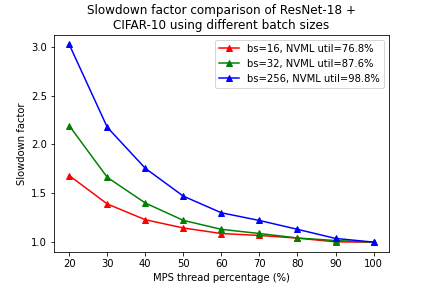
\includegraphics[width=.33\textwidth]{images/fig2_ResNet-18.png}\hfill
    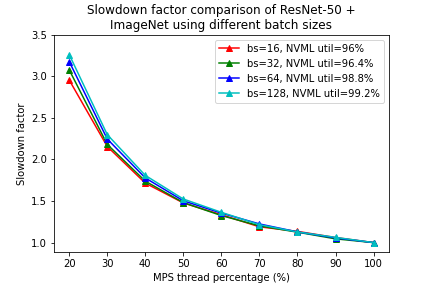
\includegraphics[width=.33\textwidth]{images/fig2_ResNet-50.png}\hfill
    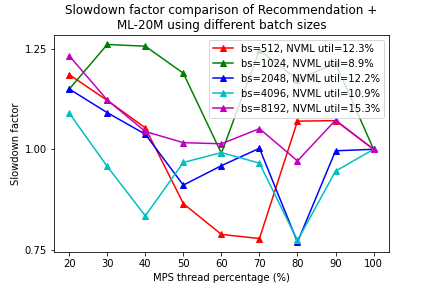
\includegraphics[width=.33\textwidth]{images/fig2_Recommendation.png}\hfill
    % \\[\smallskipamount]
    \caption{Slowdown factor comparison of different workloads. Generally, the less resource-demanding a workload is, the less resources it should be given by the scheduler to maximize the overall throughput of all jobs co-located on the same accelerator.}
    \label{fig:foobar}
\end{figure*}

\begin{table*}[t]
\label{aggressive_packing}
\vskip 0.15in
\begin{center}
\begin{small}
\begin{tabular*}{\textwidth}{@{\extracolsep{\fill}}|c|c|cc|c|}
\toprule
\# Jobs Packed & Makespan/Avg JCT & Makespan Running Sequentially & Avg JCT Running Sequentially & Total Throughput \\
\midrule
1 & 53 & 53 & 53 & 943 \\
2 & 60 & 106 & 79.5 & 1667 \\
3 & 77 & 159 & 106 & 1948 \\
4 & 96 & 212 & 132.5 & 2083 \\
7 & 150 & 371 & 212 & \textbf{2333} \\
\bottomrule
\end{tabular*}
\end{small}
\end{center}
\caption{The benefits of packing 2+ jobs concurrently. When packing N jobs concurrently, all of them start and end at roughly the same time, so they have the same makespan and avg JCT. All time units are in seconds. The unit for total throughput is img/s.}
\vskip -0.1in
\end{table*}


\subsection{Utilizations of Common DL/HPC Workloads}

In this section, using the fine-grained utilization profiler we developed on top of NVIDIA Visual Profiler, we provide a brief overview of the utilization characteristics of different types of cores in common DL/HPC workloads.

% From table \ref{common-workloads}, we confirm our finding that NVML provides an upper-bound estimate of the actual core utilizations, and there is potentially plentiful resources being wasted as a result of the traditional exclusive-access model of cluster scheduling policies.

From Table \ref{common-workloads}, we confirm our conjecture that NVML provides an inaccurate estimation of the actual utilizations with two findings: (1) The NVML Util is an upper-bound, coarse-grained estimation of the actual core utilizations. (2) For most tasks, only 1-2 types of cores are being utilized while others are idling. This indicates that there is potentially plentiful resources being wasted as a result of the traditional exclusive-access model of cluster scheduling policies.





\subsection{Space Sharing vs. Traditional Scheduling Policies}

In this section, we consider the simplest case of space-sharing two jobs on one GPU. We explore different GPU sharing options and comprehensively compare different metrics of these sharing outputs.

We demonstrate the effectiveness of MPS through two experiments. In experiment 1 (Figure \ref{ss_benefits} left \& middle), we pack workloads that use different types of cores. Job 1 imitates common HPC workloads by performing a cuBLAS DGEMM operation which mostly uses FP64 cores, while job 2 trains ResNet-18 on CIFAR10 using mostly FP32 cores. From Table \ref{common-workloads}, we can observe that these two workloads have utilizations of 76.8\% and 84.72\% as reported by NVML. Traditionally, a cluster scheduler would conclude that these two jobs both have high utilizations so it will not devise to space-share these workloads. However, by using the fine-grained profiler we developed on top of nvprof, we notice that both workloads have relatively low utilization on the task-specific cores they use. As a result, we present microbenchmarks (Table \ref{pack-different-cores}) that indicate the effectiveness of physical sharing. The traditional, exclusive-access scheduling policy will run the two workloads one at a time. If we start the jobs concurrently without enabling MPS, we get a negligible gain in the overall makespan. However, with MPS enabled, we get a 33\% decrease in the makespan and a 12.3\% decrease in the average JCT. In experiment 2 (Figure \ref{ss_benefits} right), we space-share two jobs (training ResNet-18 on CIFAR10) that both under-utilize the same type of core (FP32), and we observe similar findings in a higher core utilization and decreased makespan \& avg JCT.




\subsection{Fractional Resource Allocation Weight Tuning}

In the previous section, we showed that using MPS to aid the space sharing of concurrent jobs improves both the utilization and the makespan. In this section, we empirically show that the aforementioned metrics can be further improved by tuning the fraction of resources each job being packed gets using the set of APIs provided by MPS.

% MPS documentation p. 12

In time sharing, the portion of time each job gets allocated is usually a decision made by the scheduler after acknowledging the jobs' resource requirements. This kind of fractional time sharing allows for the flexible control of the resource allocation fraction between jobs. In space sharing, the weight control can be emulated by the MPS active thread percentage control utility. The MPS control utility provides 2 sets of commands to set/query the limit of all future MPS clients. The limit can be constrained for new clients by setting the active thread percentage for a client process. By default, the active thread percentage for all processes is 100\%. Together, these APIs allow for the maximum degree of scheduling freedom.
% 4.1.1, 4.2.5

% \ref{mps_weight_tuning}

In Table 2, we show that with further fine-tuning of the fractional weights each job gets, we can reduce the average JCT of job 1 and job 2 by 15\% without severely sacrificing the run time of job 1. We also observe a 5\% decrease in the overall makespan.

% \ref{mps_weights_figure}

In Figure 2, we present a scaling analysis on the impact of different MPS thread percentages on the slowdown factor of the throughputs for different workloads. For the same (model, dataset) configuration, a larger batch size allows the training job to better utilize the support for parallelism provided by the GPU, thus resulting in a higher resource utilization. We can observe that a job with a low resource utilization has a negligible slowdown in the throughput when it gets a smaller MPS thread percentage. Intuitively, this is because this job does not fully utilize the GPU by nature, so it will not suffer from a reduced throughput after being given a less fraction of resources. In contrast, the throughput of a job with high resource demand gets linearly reduced as we decrease the MPS thread percentage it is allocated. This finding suggests that when deciding the optimal fractional allocation, the scheduler can profile the jobs to see their utilization and assign fewer resources to low resource demanding jobs to increase the net throughput of all jobs being packed.



\subsection{Aggressive Multi-Job Space Sharing}

Traditionally, in both Gandiva \cite{gandiva} and Gavel \cite{gavel}, when space sharing is considered, only  combinations of at most two jobs will be considered, as the authors found empirically that packing a larger number of jobs concurrently rarely increases the net throughput. However, we observe that packing 2+ jobs can result in a higher net throughput and a lower avg JCT/makespan if we carefully pick the jobs and partition the resources according to demand. We present microbenchmarks that support our finding.

In this experiment (Table \ref{aggressive_packing}), for simplicity, we choose a single type of job (training ResNet-18 on CIFAR-10) to evaluate the effectiveness of aggressive multi-job space sharing. When packing N jobs, we set the MPS thread percentage each job gets to be (100/N)\% for fairness/load balancing. Within the limit allowed by the available on-device memory, we are able to pack a maximum of seven jobs and observe an increase of up to 40\% in the net throughput after relaxing the number limit of jobs packed. Furthermore, when packing seven jobs, we observe a reduction of 147\% for the makespan and 41\% for the avg JCT compared to running sequentially, and a reduction of ~30\% for the makespan compared to SOTA space sharing primitives where at most two jobs are packed. However, as we increase the number of jobs packed, we notice a slowdown in the run time of individual jobs and a sub-linear increase in the total throughput of all jobs due to resource contention and inter-job interference becoming more severe. We conclude that for jobs with low resource demands, we can relax the constraint of only packing two jobs and pack 2+ jobs aggressively to increase the GPU utilization and net throughput, particularly for scheduling objectives that aim to maximize the net throughput or minimize the makespan.


% \subsection{Theoretical Support for Space Sharing}

% The most recent scheduling frameworks like Gandiva and Gavel \cite{gandiva, gavel} already take into consideration the option of space sharing when making scheduling decisions. Gandiva states that space sharing is efficient only when the packed jobs do not exceed the GPU resources (compute \& memory) and do not adversely impact each other. However, the paper does not give a very solid theoretical support for space sharing. In this section, we develop on this intuition and use profiling applications to provide a more in-depth analysis of the theoretical support for space sharing.

% motivation: tc/non-tc time, nvprof output of core utilization









\section{Future Directions}

Future directions of this project include the following:
\begin{itemize}
    \item Developing an online job profiler that has a short profiling overhead but gives accurate estimations of the resource utilization of a job, and integrating the profiler into scheduling frameworks like Gavel to aid the scheduling policies in making the optimal allocations.
    \item Developing a policy/algorithm that outputs the optimal fractional allocation of MPS thread percentages given a set of jobs space-sharing the same GPU. The optimal fraction should optimize a specified objective, e.g. minimizing makespan.
    \item Using different metrics to monitor and evaluate the compute core usage to provide a more comprehensive study of DL/HPC workloads. For example, occupancy rate \cite{occupancy} for each CUDA kernel was used by Wavelet \cite{wavelet}.
    \item NVIDIA Multi-Instance GPU (MIG) \cite{mig} is a virtualization technique that supports latest NVIDIA GPUs. It can partition an A100 GPU into as many as seven instances, each fully isolated with their own high-bandwidth memory, cache, and compute cores. Instead of using the MPS thread percentage for coarse-grained resource partition, we can use MIG for fine-grained, precise resource partition of jobs sharing the same physical GPU.
\end{itemize}

\section{Conclusions}

In this report, we explored the effectiveness of space sharing compared with those of traditional scheduling policies. We present two techniques, namely fractional resource partition and aggressive multi-job colocation, to further increase the benefits of space sharing. We conclude that with the proper profiling of jobs, scheduling policies can make aggressive yet cautious space sharing decisions to improve both the cluster utilization and finish time of a queue of jobs. Our findings further suggest that GPU cluster scheduling policies should be aware of the resource demands of jobs to apply proper optimizations.


\vfill

\bibliography{example_paper}
\bibliographystyle{mlsys2021}

% \vfill
%%%%%%%%%%%%%%%%%%%%%%%%%%%%%%%%%%%%%%%%%%%%%%%%%%%%%%%%%%%%%%%%%%%%%%%%%%%%%%%
%%%%%%%%%%%%%%%%%%%%%%%%%%%%%%%%%%%%%%%%%%%%%%%%%%%%%%%%%%%%%%%%%%%%%%%%%%%%%%%
% SUPPLEMENTAL CONTENT AS APPENDIX AFTER REFERENCES
%%%%%%%%%%%%%%%%%%%%%%%%%%%%%%%%%%%%%%%%%%%%%%%%%%%%%%%%%%%%%%%%%%%%%%%%%%%%%%%
%%%%%%%%%%%%%%%%%%%%%%%%%%%%%%%%%%%%%%%%%%%%%%%%%%%%%%%%%%%%%%%%%%%%%%%%%%%%%%%
\appendix

\section{Replicating the results}
%
The source code and instructions to replicate all results in this report are available at:
\begin{center}
\textbf{\texttt{https://github.com/ruipeterpan/cs759-sp21}}
\end{center}

The Python package for interacting with NVIDIA MPS is open-sourced at:
\begin{center}
\textbf{\texttt{https://github.com/ruipeterpan/pymps}}
\end{center}


%%%%%%%%%%%%%%%%%%%%%%%%%%%%%%%%%%%%%%%%%%%%%%%%%%%%%%%%%%%%%%%%%%%%%%%%%%%%%%%
%%%%%%%%%%%%%%%%%%%%%%%%%%%%%%%%%%%%%%%%%%%%%%%%%%%%%%%%%%%%%%%%%%%%%%%%%%%%%%%


\end{document}


% This document was modified from the file originally made available by
% Pat Langley and Andrea Danyluk for ICML-2K. This version was created
% by Iain Murray in 2018. It was modified from a version from Dan Roy in
% 2017, which was based on a version from Lise Getoor and Tobias
% Scheffer, which was slightly modified from the 2010 version by
% Thorsten Joachims & Johannes Fuernkranz, slightly modified from the
% 2009 version by Kiri Wagstaff and Sam Roweis's 2008 version, which is
% slightly modified from Prasad Tadepalli's 2007 version which is a
% lightly changed version of the previous year's version by Andrew
% Moore, which was in turn edited from those of Kristian Kersting and
% Codrina Lauth. Alex Smola contributed to the algorithmic style files.
